\documentclass[runningheads,10pt]{llncs}

\usepackage{graphicx} % Required for inserting images
\usepackage{amsmath}
\usepackage{verbatim}
\usepackage{acro} %% acronimos 
\usepackage[utf8]{inputenc}  % Para caracteres Unicode
\usepackage{textgreek}       % Para utilizar \textmu como alternativa a \mu
\usepackage{listings} % Para mostrar código JSON en formato LaTeX
\usepackage{array}
\usepackage{soul} % Permite tachado y subrayado avanzado
\usepackage{multirow}
\usepackage{subcaption}
\usepackage{subcaption} % Para subfiguras
\usepackage{caption} % Manejo avanzado de captions
\usepackage[a4paper,margin=1in]{geometry} % Márgenes reducidos
\setlength{\tabcolsep}{2pt} % Reducir espacio entre columnas
\usepackage[tableposition=bottom, labelfont=bf, skip=20pt]{caption} % 'tableposition=bottom' para el caption debajo y 'skip' para el espacio. labelfont=bf para negritas
\usepackage[colorinlinetodo]{todonotes} % O use color todo para resaltar
\usepackage{url}
\usepackage[ruled,vlined]{algorithm2e}
\usepackage{booktabs}
\usepackage{tikz}
\usetikzlibrary{shapes, arrows, positioning}

%\usepackage{color}
%\usepackage{multicol}
%\setlength{\parindent}{0pt}

\setlength{\tabcolsep}{4pt} % Espacio horizontal en celdas
\renewcommand{\arraystretch}{1.0} % Espacio vertical en celdas

\usepackage{courier}
\usepackage{geometry}
\geometry{margin=1in}

%%\usepackage{enumitem} % Paquete para personalizar listas
% Redefinir el símbolo de itemize en todos los niveles
%% \setlist[itemize]{label=\textbullet} % Cambia el guión a un punto

%\title{Interpretability by Gram-Weighted Mapping (IGWM)}
%\title{Improving Visual Interpretability in NLP Short-Text Tasks: A Pre-Hoc Approach Based on Gram-Weighted Tracing}
%\title{Pre-Hoc Visual Interpretability in Short-Text NLP Tasks via Gram-Weighted Tracing}

\title{Gram-Weighted Tracing for Pre-Hoc Visual Interpretability in Sparse Short-Text NLP Tasks}

\titlerunning{Improving Visual Interpretability in Short-Text Classification: A Pre-Hoc Approach...}
\date{February 2025}
\author{José J. Calderón\inst{1,3} 
\and ~\\ Mario Graff\inst{1,2}
\and Eric S. Tellez\inst{1,2} 
}
\institute{INFOTEC Centro de Investigaci\'on e Innovaci\'on en Tecnolog\'ias de la Informaci\'on y Comunicaci\'on. Circuito Tecnopolo Sur No 112, Fracc. Tecnopolo Pocitos II, Aguascalientes 20313, México\\
\and
Consejo Nacional de Humanidades, Ciencias y Tecnologías (SECIHTI), Insurgentes Sur 1582, Crédito Constructor, CDMX, México\\
\email{\{mario.graff, eric.tellez\}@infotec.mx}
\and
CIMAV Center for Research in Advanced Materials. Av. Miguel de Cervantes 120 Complejo Industrial,
Chihuahua, Chih. 31136, México. \\
\email{juan.calderon@cimav.edu.mx}
}

% Incluye el archivo de acrónimos
% Definición de acrónimos



\DeclareAcronym{GWTI}{
  short = GWTI,
  long  = Gram-Weighted Tracing for Interpretability
}

\DeclareAcronym{AI}{
  short = AI,
  long  = Artificial Intelligence
}

\DeclareAcronym{XAI}{
  short = XAI,
  long  = Explainable Artificial Intelligence
}
\DeclareAcronym{NLP}{
  short = NLP,
  long  = Natural Language Processing
}

\DeclareAcronym{mTC}{
    short=$\mu\text{TC}$,
    long=Micro Text Classifier, 
}  

\DeclareAcronym{LIME}{
  short = LIME,
  long  = Local Interpretable Model-agnostic Explanations,
}

\DeclareAcronym{SHAP}{
  short = SHAP,
  long  = SHapley Additive exPlanations,
}

\DeclareAcronym{PCA}{
  short = PCA,
  long  = Principal Component Analysis,
}

\DeclareAcronym{RFE}{
  short = RFE,
  long = Recursive Feature Elimination
}  

\DeclareAcronym{SVM}{
  short = SVM,
  long  = Support Vector Machine,
}

\DeclareAcronym{ML}{
  short = ML,
  long  = Machine Learning,
}


\DeclareAcronym{LinearSVC}{
  short = LinearSVC,
  long  = Linear Support Vector Classification,
}

\DeclareAcronym{OOV}{
  short = OOV,
  long  = Out of Vocabulary,
}

\DeclareAcronym{BERT}{
  short = BERT,
  long  = Bidirectional Encoder Representations from Transformers,
}

\DeclareAcronym{TfIdf}{
  short = Tf-Idf,
  long  = Term Frequency-Inverse Document Frequency,
}

\DeclareAcronym{BoW}{
  short = BoW,
  long  = Bag of Words,
}

\begin{document}

\maketitle

\begin{abstract}

Besides traditional linguistic challenges —such as ambiguity and noise— short-text \ac{NLP} tasks like user profiling and tweet classification suffer from high dimensionality and sparsity, which severely hinder explainability in token-based models based on \ac{BoW} schemes. We present \ac{GWTI}, a pre-hoc interpretability framework that combines a linear estimator with a q-gram tracing method to generate visual, token-level explanations. \ac{GWTI} supports simultaneous analysis of all tweet instances and enables q-gram contributions to be traced back to their original words, restoring a human-understandable representation that enhances interpretability. Unlike post-hoc methods, \ac{GWTI} is applied before model training and is designed as a lightweight tool for active learning strategies, allowing iterative data refinement and dataset optimization.

\keywords{XAI, Pre-hoc Interpretability, Visual Interpretability, q-grams, NLP Short-Text Tasks, Sparse Representations, Token Contribution Analysis, Active Learning}

\end{abstract}

\section{Introduction}
\label{sec/introduction}

Short-text classification and user profiling tasks, particularly those involving tweets, present unique challenges for both model performance and interpretability~\cite{zhao2024explainability}. These challenges arise not only from linguistic issues like ambiguity, noise and lack of context~\cite{yadav2021comprehensive,ashfaq2021natural,wang2021hierarchical}, but also from structural factors, such as high dimensionality and sparsity in \ac{BoW} representations caused by the presence of a high number of unique words in very few tweets~\cite{chen2022multiple,pattanayak2024semi}. The sparse nature of short texts—where most terms appear infrequently—complicates the attribution of importance to individual tokens, limiting human-understandable explanations~\cite{wang2021hierarchical}.

To address these issues, we propose \ac{GWTI}, an interpretability framework based in a pre-hoc explainability model~\cite{zhao2024explainability} that leverages q-gram tokenization~\cite{tellez2017case,hacohen2020influence} and linear estimator to deliver token-level visual explanations. While q-grams are effective in capturing morphological variation and handling out-of-vocabulary terms, they often generate fragmented and hard-to-interpret features. \ac{GWTI} solves this by tracing each q-gram back to its originating word, enabling intuitive visualizations that preserve model performance and enhance human interpretability.

By integrating interpretability into the preprocessing stage—before model training—\ac{GWTI} supports strategies such as active learning, domain adaptation, and error analysis. It is designed as a lightweight framework that combines q-gram-based tokenization with interpretable linear modeling and a novel tracing mechanism, enabling token-level visualizations that are both scalable and human-readable. In this work, we introduce the \ac{GWTI} framework, evaluate its ability to enhance interpretability in sparse, short-text \ac{NLP} tasks, and compare its performance against post-hoc methods such as \ac{SHAP} and \ac{LIME}. Additionally, we demonstrate its use in practical scenarios involving dataset refinement, token-level bias detection, and model debugging across multiple corpora of tweets.

\section{State of the Art}
\label{sec/state-of-the-art}

\subsection{Q-gram Tokenization}
Q-grams are overlapping sequences of characters extracted from words. Their tolerance to typographical errors and resilience to informal language make them particularly effective in short-text \ac{NLP} tasks such as tweet classification and user profiling \cite{tellez2017case,hacohen2020influence}. By decomposing words into subword units, q-grams offer improved handling of slang, neologisms, and out-of-vocabulary terms. However, these fragmented features lack semantic coherence, making their contribution to model decisions difficult to interpret without auxiliary mechanisms.

Figure~\ref{fig:q_gram_tokenization} shows a basic example of q-gram tokenization (\textit{q} = 2) using \ac{mTC}. The phrase \textit{hello word} is tokenized into overlapping 2-grams. This representation enhances robustness against typographical variation while fragmenting semantic structure, which motivates traceability mechanisms like \ac{GWTI}.

\begin{figure}[h]
  \centering
  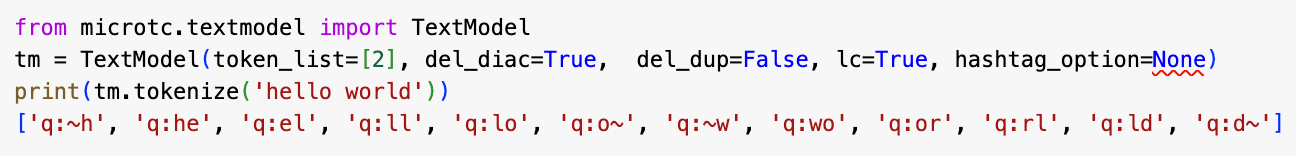
\includegraphics[width=0.95\textwidth]{q-gram_tokenization.png}
  \caption{Basic example of q-gram tokenization (\textit{q} = 2) using \ac{mTC}.}
  \label{fig:q_gram_tokenization}
\end{figure}


\subsection{Motivating the Use of Q-grams}

To justify the use of q-gram tokenization over traditional word-level approaches, we conducted a preliminary two-stage experiment. In the first stage, a classifier was trained using \ac{BoW} features derived from standard word-level tokens; in the second stage, the same setup was repeated but with q-gram tokenization. Figure~\ref{fig:comparison_qgrams} visualizes the results of this comparison through a scatter plot where each point corresponds to the F1-score of a model trained on a specific dataset. The \textit{x}-axis represents performance under word-level tokenization, while the \textit{y}-axis reflects q-gram performance. Points above the diagonal indicate improvement, whereas those below signal a decline.

The distribution pattern observed in the plot highlights a consistent trend favoring q-grams, corroborating prior findings~\cite{tellez2017case,hacohen2020influence} and underscoring their effectiveness for mitigating linguistic variability and sparsity. This empirical evidence justifies integrating q-grams into our framework as a lightweight yet powerful strategy for short-text classification.

%However, these improvements come with a trade-off: q-grams produce fragmented features that hinder interpretability—underscoring the need for frameworks like \ac{GWTI}, which recover semantic coherence by mapping q-grams back to their original words.

\begin{figure}[h]
  \centering
  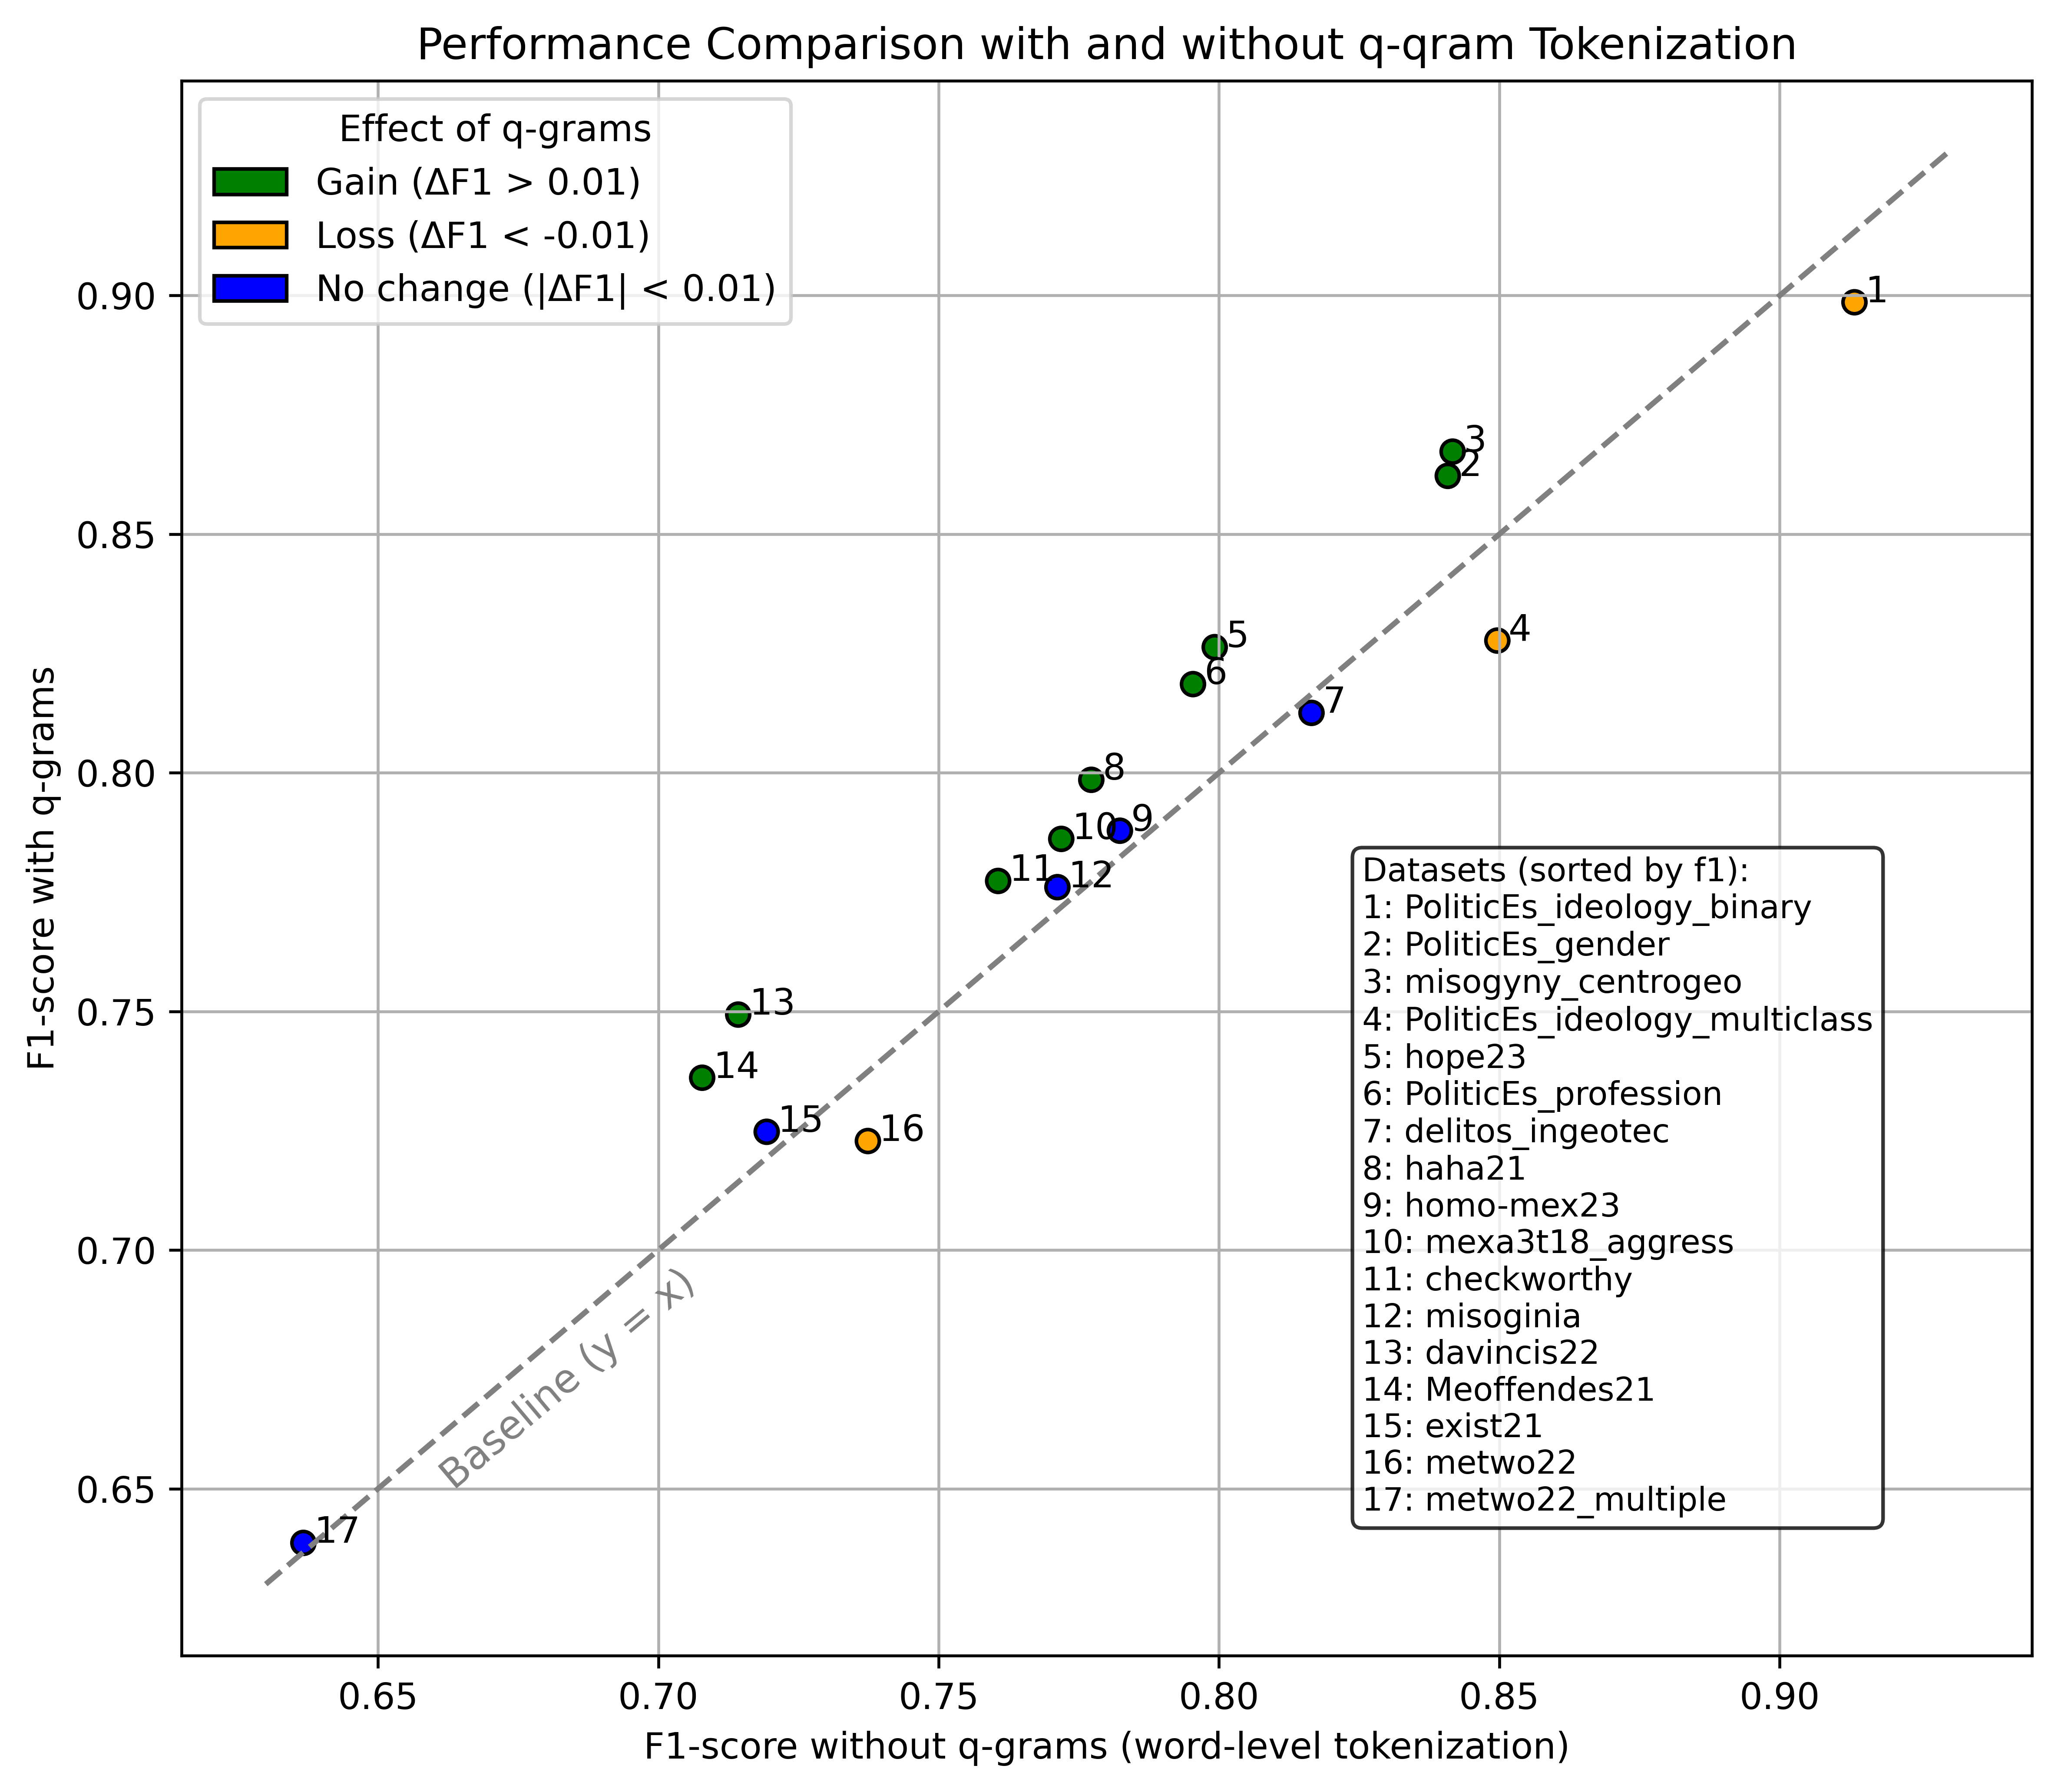
\includegraphics[width=0.75\textwidth]{comparison_qgrams.png}
  \caption{ Each point shows the F1-score of a model on a given dataset, with and without q-gram tokenization. The \textit{x}-axis corresponds to word-level tokenization (baseline), and the \textit{y}-axis to q-gram tokenization. The diagonal line (\textit{y = x}) marks equal performance. Points above indicate improvement; points below, performance loss. Overall, the distribution suggests a general tendency toward improved performance when using q-grams.}
  \label{fig:comparison_qgrams}
\end{figure}

\begin{comment}
\begin{figure}[h]
  \centering
  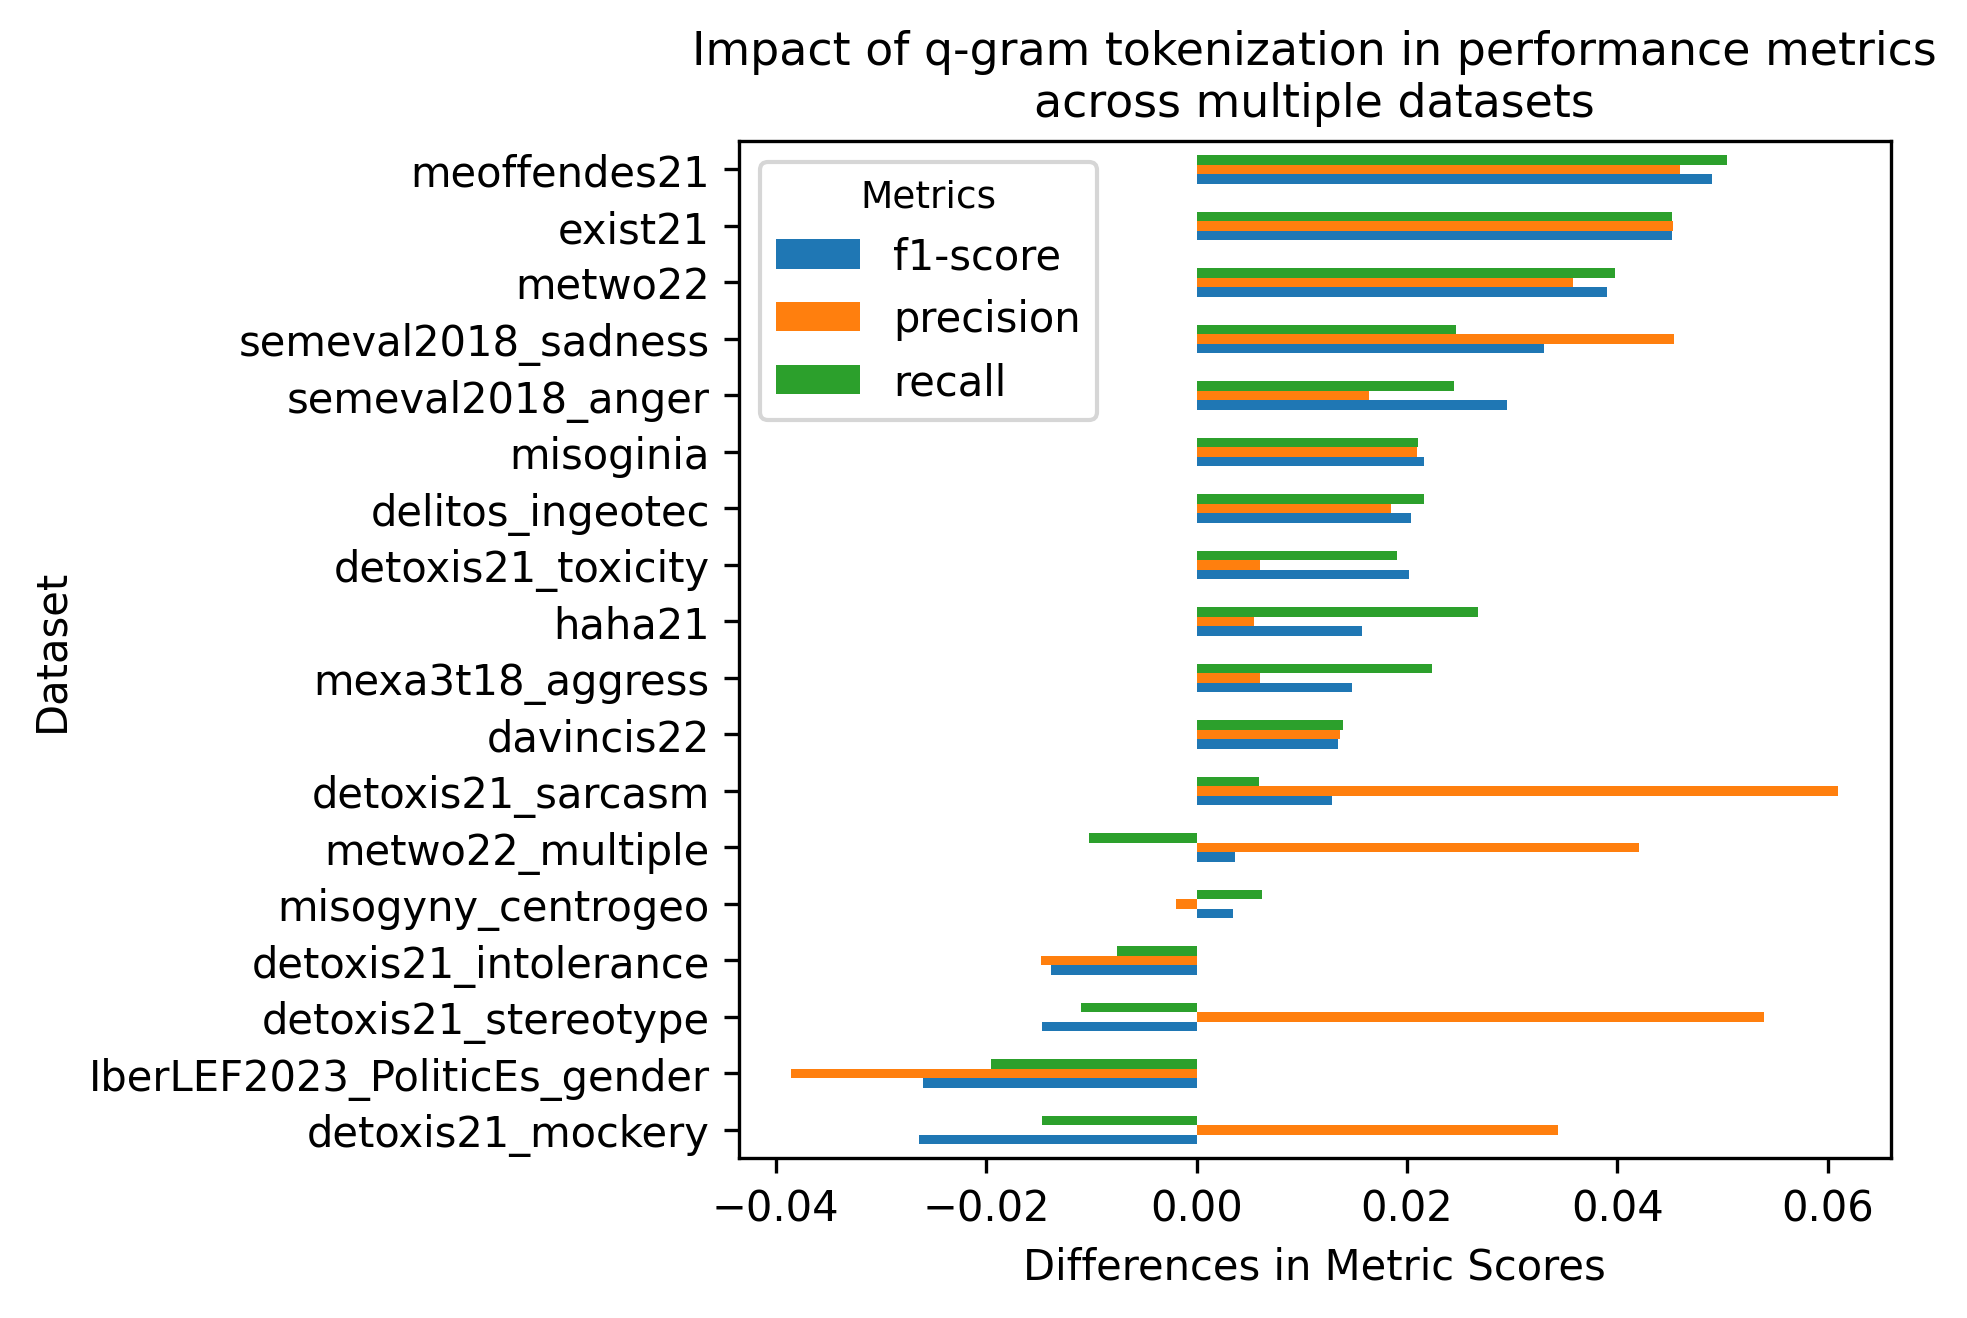
\includegraphics[width=0.85\textwidth]{metrics_qgrams.png}
  \caption{Differences in performance metrics observed after applying q-gram tokenization to \ac{NLP} datasets. The experiment involved two stages: first, tokenization was performed without q-grams to establish a baseline; then, q-gram tokenization was applied. The values plotted represent the difference or delta in each metric (f1-score, precision and recall) for each dataset, relative to the baseline. Positive values indicate improvement, while negative values suggest a performance drop.}
  \label{fig:metrics_qgrams}
\end{figure}
\end{comment}

\subsection{Challenges in Sparse and High-Dimensional Representations}

Traditional \ac{BoW} representations often lead to high-dimensional and sparse feature spaces, especially in social media data, where vocabulary is diverse and text length is limited~\cite{aminimotlagh2022reliable}. While weighting schemes such as \ac{TfIdf} mitigate this sparsity, they do not enhance the interpretability of individual tokens, particularly when working with subword units like q-grams~\cite{wang2021hierarchical}.

\subsection{Dimensionality Reduction and Feature Selection}

To address sparsity, feature selection and dimensionality reduction techniques are often applied, including L1 regularization, mutual information, and chi-square tests~\cite{heidary2024performance}. While effective in reducing complexity, these techniques may discard locally informative features and can obscure instance-level interpretability.

\subsection{Visual Explainability in \ac{NLP}}

Visual tools such as heatmaps, t-SNE, and UMAP projections are effective and commonly used to interpret high-dimensional data~\cite{peeters2021exploring,do2021generalization}. However, their effectiveness diminishes when the features are excessively granular, as in the case of character-level representations. They also struggle to convey token-level decisions in a concise, human-readable form.

\subsection{Post-hoc Explainability: Strengths and Weaknesses}
\label{post-hoc-strengths}

Post-hoc methods such as \ac{SHAP} and \ac{LIME} have gained widespread use in interpreting model predictions. \ac{SHAP} computes feature contributions based on Shapley values, while \ac{LIME} fits a local interpretable model around the prediction instance. Despite their utility, both methods suffer performance degradation in high-dimensional feature spaces—such as those produced by q-gram tokenization—due to increased computational cost, approximation instability, and cluttered visualizations. In sparse short-text datasets, the number of features can exceed thousands, making individual token attributions noisy and less informative.

Figure~\ref{fig:shap_visual} illustrates a typical \ac{SHAP} explanation over a tweet instance. The visualization is composed of two plots. The first shows \ac{SHAP} values computed over a word-level \ac{BoW} representation, where the limited number of tokens allows for a clear display of their relative contributions. The second shows the same tweet processed with q-gram tokenization. In this case, \ac{SHAP} attempts to render over 100 q-gram features, leading to an unreadable visualization and fails to provide coherent semantic insights at the word level complicating. This highlights the limitations of post-hoc tools in sparse, high-dimensional contexts.

\begin{figure}[ht]
    \centering
    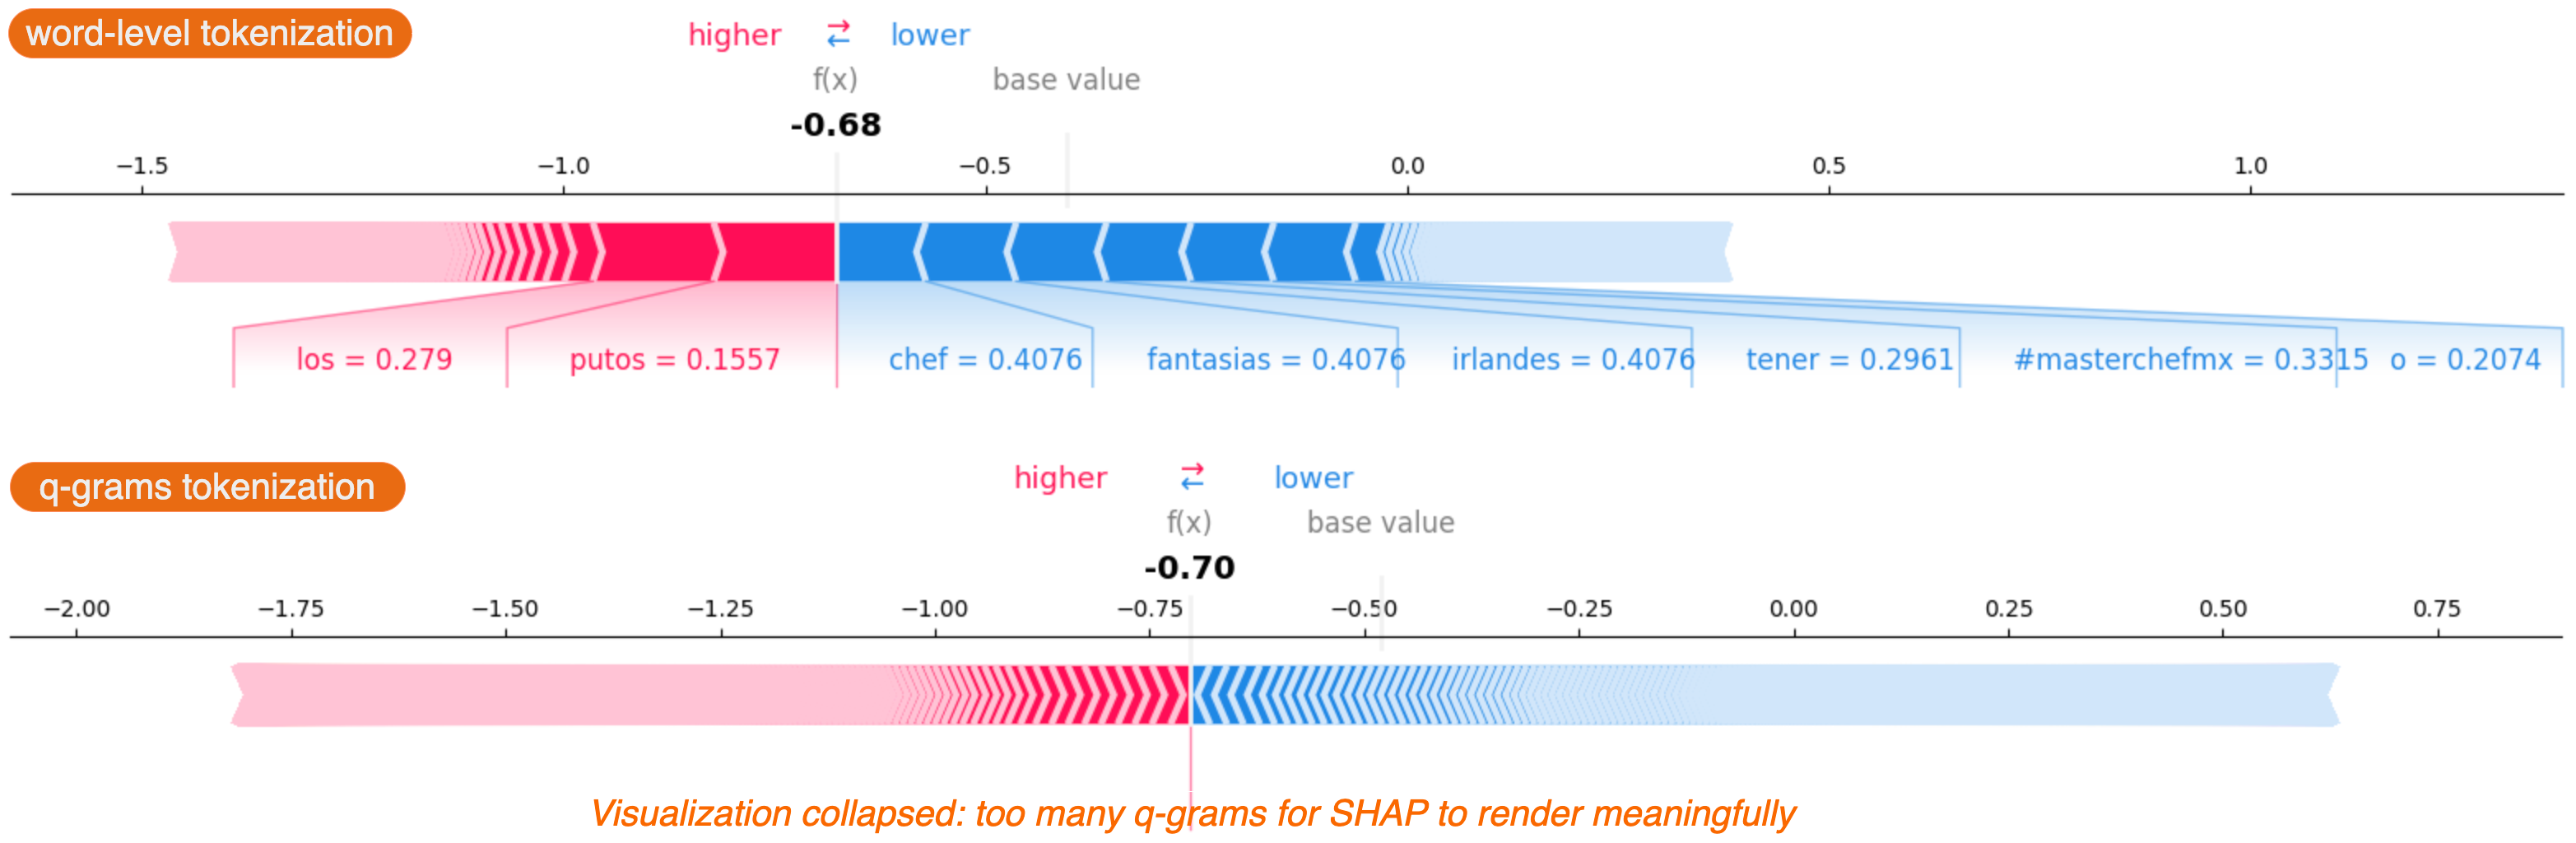
\includegraphics[width=0.95\textwidth]{shap-instance.drawio.png}
    \caption{\ac{SHAP} visualization for the same tweet instance: word-level tokens (top) vs. q-grams (bottom). High dimensionality in the q-gram representation prevents effective visualization, hinder human interpretation.}
    \label{fig:shap_visual}
\end{figure}

\subsection{Pre-hoc vs Post-hoc Approaches}

Interpretability in machine learning can be integrated either before or after training. Pre-hoc approaches embed explainability directly into the model design, typically using interpretable models like linear classifiers or decision trees~\cite{gilpin2018explaining}. These models offer transparency by construction, allowing feature contributions to be extracted and visualized without approximation.

In contrast, post-hoc approaches—such as \ac{SHAP} and \ac{LIME}—interpret the predictions of any trained model by approximating its behavior locally~\cite{salih2023commentary}. Although model-agnostic and widely applicable, they often suffer from instability, high computational cost, and difficulties when handling high-dimensional input spaces, such as those produced by q-gram tokenization.

While hybrid approaches have emerged to combine the flexibility of post-hoc tools with the transparency of pre-hoc models, they are typically more complex and harder to scale~\cite{biswas2024hybrid}. In scenarios involving short-text classification with sparse, noisy data, pre-hoc strategies remain a more reliable and efficient option.

\subsection{Motivation for \ac{GWTI}}
Building on this context, \ac{GWTI} combines the robustness of q-grams with the inherent interpretability of linear models, while introducing a tracing mechanism that links q-grams back to their original words. This mechanism restores semantic coherence and supports visual explanations that are both interpretable and scalable. Unlike post-hoc techniques, \ac{GWTI} operates before training, making it suitable for use in data refinement, active learning, and exploratory analysis within short-text pipelines.

\section{Methodology}
\label{sec/methodology}

This section presents the full architecture and rationale of the proposed \ac{GWTI} framework. \ac{GWTI} is designed to address the challenge of interpretability in short-text classification, particularly in sparse and high-dimensional scenarios resulting from q-gram tokenization. The framework integrates lightweight computation, visual interpretability, and token-level tracing. Below, we detail each component.

\subsection{Datasets}

We evaluate \ac{GWTI} using tweet datasets, annotated for user profiling and classification tasks. These datasets were released as part of shared evaluation campaigns under the IberLEF\footnote{IberLEF: Iberian Languages Evaluation Forum} and CLEF\footnote{CLEF: Conference and Labs of the Evaluation Forum} initiatives, which offer high-quality annotations and well-defined evaluation protocols. Using competition datasets reduces the need for collecting and labeling tweets manually, saving substantial effort while ensuring task realism and reproducibility.

Each dataset presents challenges typical of short-text \ac{NLP}, including informal language, high lexical diversity, and label imbalance. For user profiling, we apply unsupervised clustering using k-means to group users into profile categories, allowing the framework to generalize to new profiling tasks.

\subsection{Text Transformation with \ac{mTC}}

After dataset selection, the next step in the \ac{GWTI} pipeline is transforming the raw tweet texts into numerical vectors suitable for training interpretable models. This transformation is performed using \ac{BoW} schemes, which rely on a fixed vocabulary of tokens to represent documents as sparse vectors. In our case, the tokens are derived from overlapping character sequences—q-grams—rather than full words.

This tokenization strategy introduces two technical requirements: first, the transformation must efficiently support q-gram fragmentation across thousands of short texts; second, it must preserve information about the frequency and distribution of these subword units to enable downstream interpretability. To meet these needs, we selected the \ac{mTC} framework, which is specifically optimized for short-text vectorization and classification.

\ac{mTC} offers robust support for character-level tokenization, \ac{TfIdf} vector construction, and integration with popular linear classifiers such as \ac{LinearSVC}. It allows for direct generation of vector-label pairs from annotated datasets, accelerating experimentation and simplifying preprocessing. This makes possible to build our q-gram tracing mechanism directly on top of the \ac{mTC} output, ensuring that every visual explanation can be linked back to a semantically meaningful word. The resulting \ac{TfIdf} vectors form the basis for visual interpretation.

\subsection{Dimensionality Reduction and Feature Selection}

Q-gram tokenization often produces thousands of features, increasing both dimensionality and sparsity. These features correspond to fragmented character-level n-grams rather than semantically complete tokens. To address this, we employ L1 regularization during training, promoting sparsity by reducing less informative q-gram features to zero. This enhances model interpretability, preserves the efficiency of computation, and reduces overfitting.

\subsection{Integration of an Interpretable Linear Model (LinearSVC)}

The core estimator in \ac{GWTI} is a \ac{LinearSVC} implemented by the Scikit-learn library \cite{scikit-learn}. It is well-suited for high-dimensional, sparse data, offers low computational cost and direct access to learned coefficients. \ac{LinearSVC} is a linear classification model that seeks to find the hyperplane that best separates the classes by maximizing the margin between them. Its learned coefficients are especially valuable for interpretability, as they indicate the contribution of each q-gram feature to the classification decision.

These coefficients allow us to easily define a threshold below which q-gram contributions can be considered negligible, thus reducing noise in visual explanations. This mechanism does not require any additional computation beyond standard training and is independent of the downstream prediction process or target model.

All these characteristics are aligned with the goals of \ac{GWTI}, which focuses on interpretability for NLP tasks, particularly in sparse, short-text contexts where token-level decisions must be explained clearly and efficiently. The combination of μTC’s deterministic q-gram vectorization with LinearSVC’s sparse, interpretable modeling results in a seamless and computationally efficient pipeline. This synergy enables \ac{GWTI} to deliver clear, token-level visualizations that are both scalable and grounded in formally justified model behavior. 

Particularly, the consistency and traceable of μTC’s q-gram vectorization is fundamental for \ac{GWTI}, as it ensures that each vector dimension corresponds reliably to a specific subword unit. This alignment makes it possible to map the classifier’s learned coefficients back to their original text fragments without ambiguity, supporting faithful and deterministic token-level explanations.

\begin{comment}
\subsection{GWTI Framework Workflow}
The GWTI framework follows a streamlined six-stage pipeline (Figure~\ref{fig:GWTI_flow}):

\begin{itemize}
    \item \textbf{Input Text Processing}: Raw tweets are normalized while preserving original token boundaries
    \item \textbf{$\mu$TC Tokenization}: Words are decomposed into overlapping q-grams ($q\in\{2,3,4\}$)
    \item \textbf{TF-IDF Weighting}: Q-grams receive importance scores based on corpus statistics
    \item \textbf{Linear Classification}: A sparse LinearSVC model learns q-gram coefficients
    \item \textbf{Q-gram-to-Word Tracing}: Our novel tracing mechanism aggregates subword contributions
    \item \textbf{Visual Explanation}: Words are color-coded by their influence on predictions
\end{itemize}
\end{comment}

\subsection{Workflow - Token-Level Interpretability via Q-Gram Tracing}

The GWTI framework operates through a streamlined, six-stage pipeline that enables end-to-end interpretability for short-text classification tasks. Figure~\ref{fig:GWTI_flow} summarizes this process, while Algorithm~\ref{alg:tracing} formalizes the complete procedure.

\subsubsection{Workflow}

\begin{enumerate}
    \item \textbf{Input Text Processing:} Raw tweets are normalized while preserving original token boundaries.
    \item \textbf{\textmu TC Tokenization:} Words are decomposed into overlapping q-grams ($q \in \{2, 3, 4\}$).
    \item \textbf{TF-IDF Weighting:} Q-grams are assigned weights based on corpus-level statistics.
    \item \textbf{Linear Classification:} A sparse LinearSVC model learns the coefficients for each q-gram.
    \item \textbf{Q-gram-to-Word Tracing:} Our novel tracing mechanism aggregates subword contributions to recover word-level relevance.
    \item \textbf{Visual Explanation:} Tokens are color-coded by their influence on the model’s predictions.
\end{enumerate}

\begin{figure}[h]
\centering
\begin{tikzpicture}[
    node distance=0.90cm,
    box/.style={draw, rectangle, minimum height=0.7cm, minimum width=1.8cm, align=center, fill=blue!10, rounded corners, font=\footnotesize},
    arrow/.style={->, >=stealth, semithick},
    label/.style={font=\small, align=center} %scriptsize
]

\node[box] (input) {Input};
\node[box, right=of input] (token) {$\mu$TC \\ q-grams};
\node[box, right=of token] (tfidf) {TF-IDF};
\node[box, right=of tfidf] (model) {LinearSVC};
\node[box, right=of model] (trace) {Trace \\ q-grams};
\node[box, right=of trace] (output) {Viz};

\foreach \from/\to in {input/token, token/tfidf, tfidf/model, model/trace, trace/output} 
    \draw[arrow] (\from) -- (\to);

\node[below=0.1cm of input, label] {raw text};
\node[below=0.1cm of token, label] {subword\\tokens};
\node[below=0.1cm of tfidf, label] {weighted\\features};
\node[below=0.1cm of model, label] {coefficients};
\node[below=0.1cm of trace, label] {word-level\\mappings}; 
\node[below=0.1cm of output, label] {color-coded\\explanations};

\end{tikzpicture}
\caption{Workflow of the GWTI framework: (1) Input text processing, (2) μTC tokenization, (3) TF-IDF weighting, (4) Linear classification, (5) q-gram-to-word tracing, and (6) visual explanation generation.\\
Overview of the GWTI pipeline: from raw text to color-coded token-level visual explanations.}
\label{fig:GWTI_flow}
\end{figure}

Step 5 represents GWTI’s core innovation: it bridges the gap between fragmented q-gram features and human-interpretable words through a deterministic reconstruction process. This approach proves highly effective in sparse, short-text scenarios as demonstrated in Section~\ref{sec:experiments}.

Algorithm~\ref{alg:tracing} spans from preprocessing to visual rendering, maintaining semantic coherence, low computational complexity, and full traceability across all stages.


\subsection{Algorithm - Token-Level Interpretability via Q-Gram Tracing}

A major interpretability challenge of using q-gram representations is their lack of semantic coherence: q-grams are fragments of words and cannot be directly understood without reconstructing their context. \ac{GWTI} addresses this challenge by implementing a tracing mechanism that reestablishes a human-readable interpretation of model decisions at the word level.

The tracing process begins by iterating over each tweet and extracting the \ac{TfIdf} weights of the q-grams. These are then matched with the global model coefficients learned by the classifier. For each word in the tweet, the algorithm performs a new tokenization using the same q-gram scheme and parameters applied during training. Thanks to μTC’s determinism, the same q-grams are reliably regenerated, and their contributions (\ac{TfIdf} × coefficient) are accumulated to compute a word-level score.

This strategy ensures a lightweight and deterministic aggregation of q-gram contributions, enabling the construction of heatmaps that visually encode the influence of each word on the model's decision. However, the tracing mechanism evaluates each word in isolation. It does not consider overlapping q-grams between words nor q-gram skip patterns across boundaries, which are capabilities supported by the underlying \ac{mTC} tokenization but intentionally excluded from the interpretability mechanism to maintain computational simplicity.

As a result, the approach trades some expressive power for speed and clarity: it sacrifices inter-word contextual interactions to preserve efficient, per-word explainability. This constraint limits the reconstruction of complex linguistic structures but suffices to produce human-interpretable, token-level insights in short, sparse texts like tweets.

Algorithm~\ref{alg:tracing} outlines the complete procedure.

\begin{algorithm}[ht]
\caption{Q-Gram-Based Interpretability Framework}
\label{alg:tracing}
\KwIn{Tweet dataset $D$, parameters: sample size $s$, decision threshold $\theta$, weight threshold $\tau$}
\KwOut{Visualization-ready interpretability structure}

\textbf{Step 1: Data Input and Configuration} \\
Load dataset $D$; configure parameters $\{s, \theta, \tau\}$

\textbf{Step 2: Preprocessing and Tokenization} \\
\ForEach{tweet $t \in D$}{
    Tokenize $t$ into words and q-grams ($q \in \{2,3,4\}$)\;
    Compute TF-IDF weights $x_g$ for each q-gram $g$ in $t$\;
}

\textbf{Step 3: Feature Selection and Dimensionality Reduction} \\
Apply Mutual Information or Chi-Square to select top-$k$ informative tokens

\textbf{Step 4: Train Linear Model} \\
Fit LinearSVC on selected features to obtain weight vector $\mathbf{w}$ and bias $b$

\textbf{Step 5: Apply L1 Regularization} \\
Discard tokens where $|w_g| < \tau$

\textbf{Step 6: Compute Decision Scores and Classify} \\
\ForEach{instance $x$}{
    Compute $Score(x) = \sum_g x_g \cdot w_g + b$\;
    Predict class: $1$ if $Score(x) > \theta$, else $0$\;
}

\textbf{Step 7: Q-Gram Tracing to Words (Per Tweet)} \\
\ForEach{word $w_i$ in tweet $t$}{
    \State Generate q-grams $\{g_{ij}\}$ from $w_i$ using same scheme as in Step 2\;
    \State $s_i \gets \sum_{j} x_{g_{ij}} \cdot w_{g_{ij}}$ \Comment{Aggregate contribution per word}
}
\textbf{Step 8: Build Interpretability Structure} \\
\ForEach{tweet $t$}{
    Store predicted class, score, token contributions, and word mappings\;
    Save structure for visualization
}

\textbf{Step 9: Visualize Results} \\
Render heatmaps of token and word-level relevance using $\{s_i\}$\;
Display words colored by influence
\end{algorithm}


\begin{comment}
\textbf{Step 2: Preprocessing and Tokenization} \\
\ForEach{tweet $t \in D$}{
    Tokenize $t$ into words and q-grams ($q \in \{-1, 2, 3, 4\}$)\;
    Compute TF-IDF weights for each token\;
}
\textbf{Step 7: Q-Gram Tracing to Original Words} \\
\ForEach{q-gram $g$}{
    Map $g$ back to its originating word(s) in $t$
}
\end{comment}

This algorithm facilitates efficient data analysis and enables quick access to adjust or validate interpretation outcomes. Each step of Algorithm~\ref{alg:tracing} incurs predictable computational costs. Given $N$ tweet instances, average length $L$, and $q$ q-gram sizes  (e.g., $q \in \{2, 3, 4\}$), tokenization and q-gram tracing (Steps 2 and 7) scale as $\mathcal{O}(N \cdot L \cdot q)$. The construction of sparse TF-IDF vectors (Step 2) requires $\mathcal{O}(N \cdot F)$, where $F$ is the number of unique q-grams. Feature selection and model training with L1 regularization (Steps 3–5) are performed in $\mathcal{O}(I \cdot F \cdot N)$, with $I$ denoting the number of solver iterations. The scoring and classification step (Step 6) also operates in $\mathcal{O}(N \cdot F)$. Finally, the interpretability structure and visualizations (Steps 8–9) scale linearly with $\mathcal{O}(N \cdot L)$. Overall, the full \ac{GWTI} pipeline exhibits a total computational complexity of:
\[
\mathcal{O}(N \cdot L \cdot q + I \cdot F \cdot N),
\]
which ensures scalability and low overhead in short-text \ac{NLP} workflows.

Additionally, the structure generated by \ac{GWTI} is fully downloadable in JSON format, making it highly reusable and adaptable for further research. Its organized design allows researchers to extract, transform, and integrate the interpretability output into other studies or pipelines without additional effort. Appendix~\ref{ap:example_structure} shows an example of the generated structure.

\subsection{Interactive Web-Based Framework}

As part of the innovation and practical application of the proposed \ac{GWTI} framework, an interactive web-based platform has been developed that allows researchers to upload and analyze datasets of tweets for user profiling tasks, supervised classification, or related short-text \ac{NLP} tasks. This platform displays results directly on screen, enabling detailed visual analysis of each tweet alongside its predicted and pre-labeled classification.

The framework organizes and presents the data in a multi-level structure, including the decision function, true and predicted classes, and q-gram contributions. Token importance is visualized using color-coded heatmaps, while users can dynamically adjust key parameters such as the decision threshold (used to control which instances are displayed) and the weight threshold (used to filter token relevance) to refine the output.

This interactive platform supports active learning workflows by allowing users to iteratively adjust thresholds, immediately observe effects on model interpretability, and fine-tune the dataset accordingly. The output structure is downloadable in JSON format, facilitating reuse for downstream tasks or integration into alternative machine learning pipelines.

The \ac{GWTI} framework is designed for users familiar with the target model and domain, ensuring experimental control while enhancing transparency. Appendix~\ref{ap:user_interface} shows a screenshot of the interface and highlights the main features available for interactive analysis.

\todo{referencia al web-based platform}

\section{Experiments and Results}
\label{sec:experiments}

This section presents a comprehensive evaluation of \ac{GWTI}’s interpretability capabilities through three complementary perspectives. First, we showcase visual examples of token-level explanations produced by the framework. Second, we provide a quantitative experiment comparing traditional word-level modeling with our q-gram tracing approach. Finally, we contrast \ac{GWTI} with popular post-hoc interpretability methods such as \ac{SHAP} and \ac{LIME}, emphasizing the advantages of pre-hoc interpretability in sparse, high-dimensional settings.

\subsection{Visual Examples of Interpretability}

Figure~\ref{fig:tweet_instance} illustrates \ac{GWTI}'s explanation for a tweet from the MeOffendEs dataset. The heatmap highlights word-level contributions, aggregated from the associated q-grams. Red indicates positive influence (offensive), and blue negative (non-offensive). Notably, tokens such as \textit{estúpida} and \textit{mierda} show high offensive contribution, whereas \textit{altere} is non-offensive. The token \textit{talento!}, although present in the tweet, is excluded due to its low model weight, despite having high local TF-IDF—this showcases how \ac{GWTI} filters noise through weight-based thresholds.

\begin{figure}[h]
  \centering
  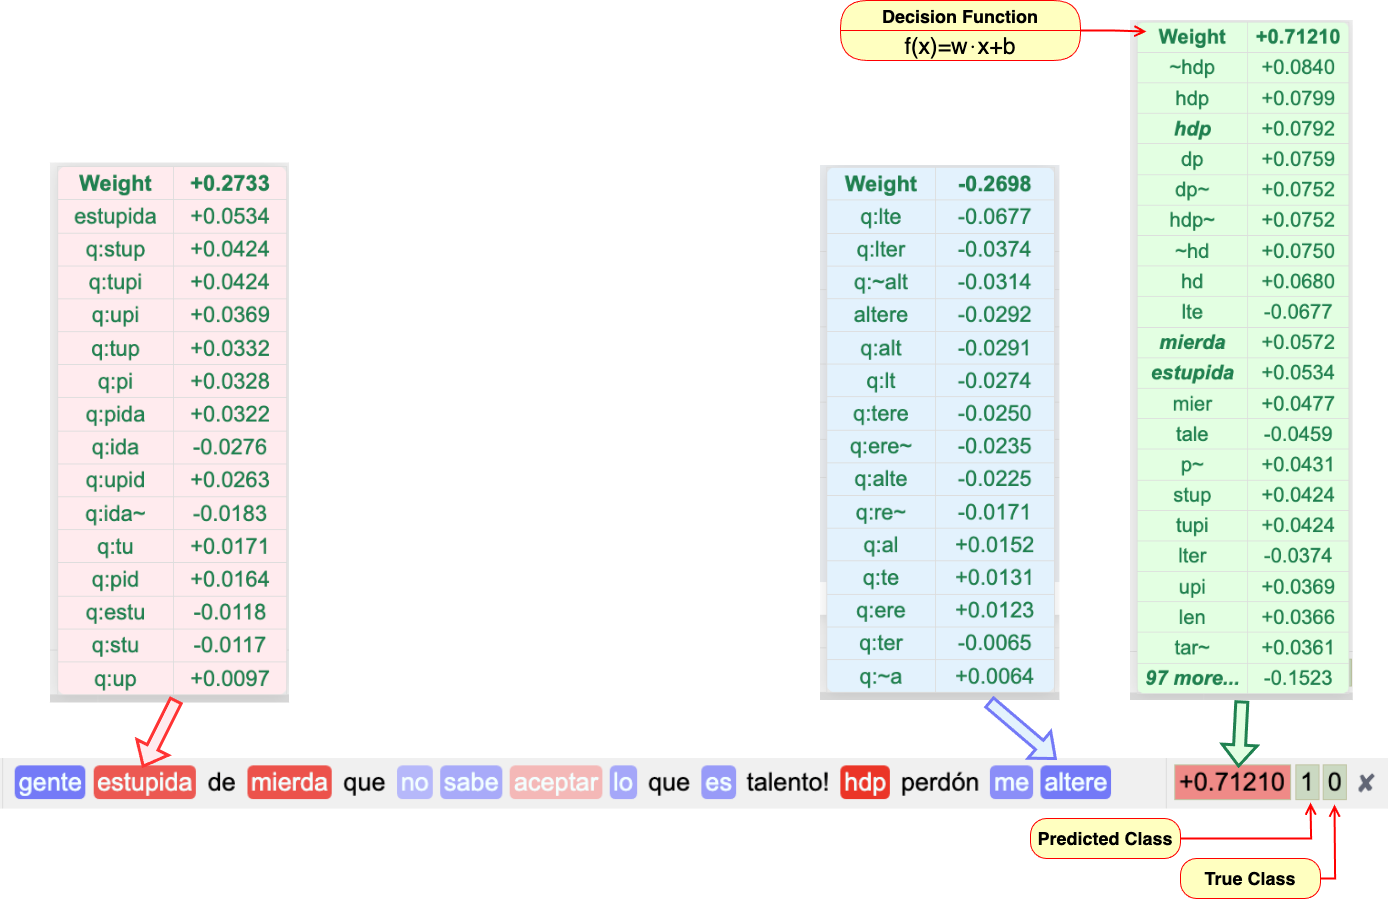
\includegraphics[width=0.9\textwidth]{tweet_sample_77.drawio.png}
  \caption{Example tweet with heatmaps indicating token importance through color intensity: red for positive (offensive) tokens and blue for negative (non-offensive) tokens. Detailed breakdown of the q-grams and their weights for the tokens \textit{estupida} and \textit{altere}, as well as an analysis of all q-grams (117 in total) in the tweet alongside the calculated decision function.}
  \label{fig:tweet_instance}
\end{figure}

The q-gram tracing mechanism is responsible for making subtle word-level contributions visible: a word like \textit{altere} may individually contribute little, but the sum of its q-grams crosses the relevance threshold. The decision function score is also displayed to indicate the confidence level of the prediction.

Figure~\ref{fig:profile_instance} shows an instance of user profiling with grouped tweets. Each tweet is rendered as a segment with annotated tokens, and the full profile displays aggregated interpretability data, including predicted and true labels. This corpus-level view is especially useful in tasks like user characterization or bias detection, as it reveals patterns across instances.

Unlike global interpretability tools limited to a few features or instances, \ac{GWTI} scales to full datasets. Token importance and selection are regulated by threshold parameters, making the system flexible for a variety of interpretability tasks.

\begin{figure}[h]
  \centering
  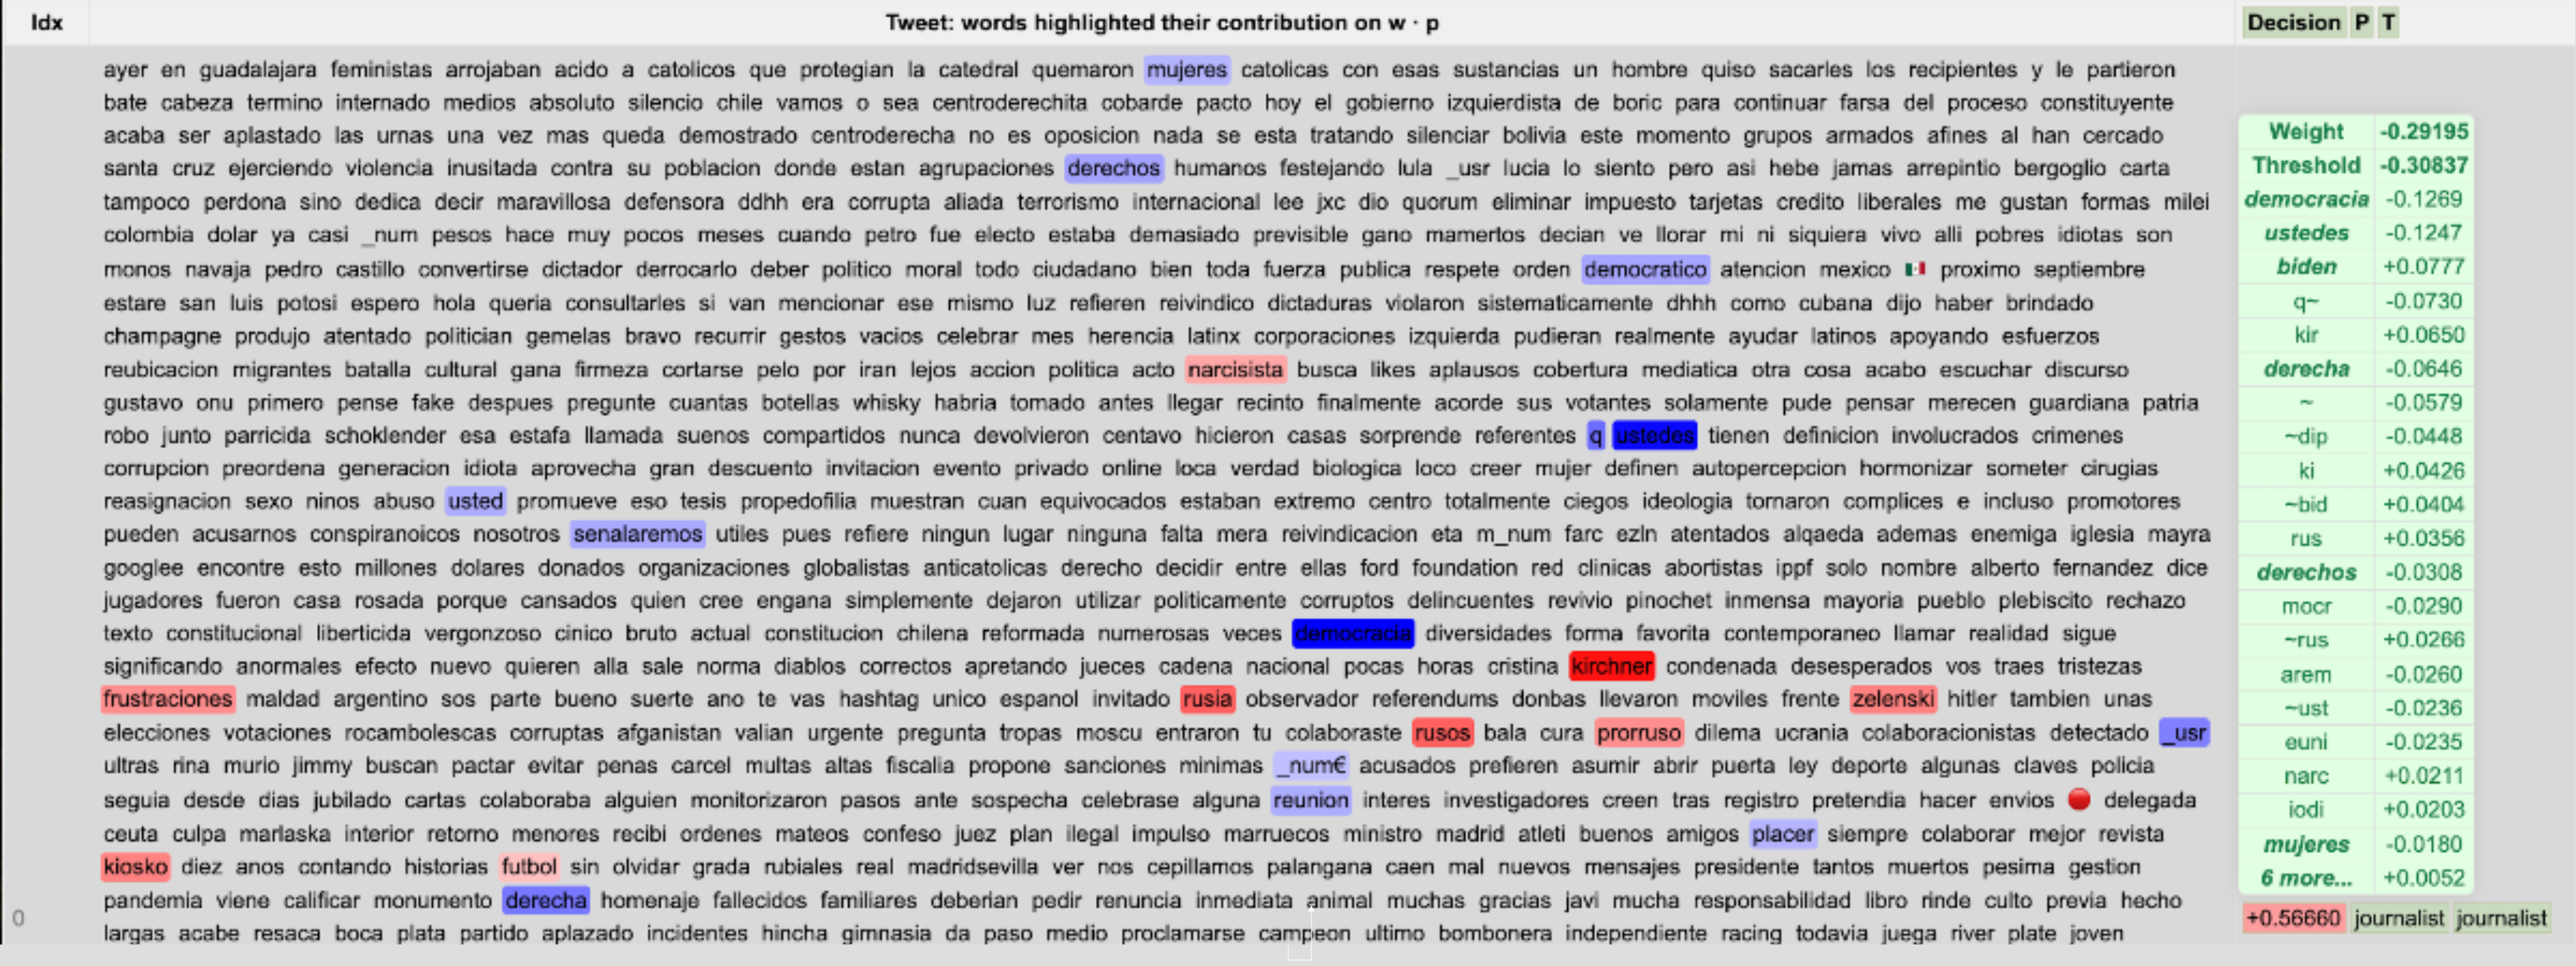
\includegraphics[width=0.99\textwidth]{user_profile_instance.png}
  \caption{Visualization of a specific instance for user profiling. This instance displays the grouped tweets for a user and the contribution of each token, facilitating the interpretation of the prediction. In this way, the \ac{GWTI} framework allows for the explainability analysis of all instances in the dataset. Appendix \ref{ap:user_interface} includes a representative segment featuring multiple tweet instances processed by the framework.}
  \label{fig:profile_instance}
\end{figure}

\subsection{Experimental Evaluation of Traceability}
To test \ac{GWTI}’s traceability effectiveness, we compare word-level feature weights against the aggregated weights of constituent q-grams across three datasets. The hypothesis is that q-gram aggregation enhances interpretability by raising more tokens above the threshold for relevance. This hypothesis assumes that the mapping of q-grams back to their parent words reveals influential patterns that are otherwise hidden when words are treated as atomic units.

We trained LinearSVC models using two representations: (1) standard tokenization with word-level TF-IDF, and (2) q-gram TF-IDF (bigrams, trigrams, 4-grams). For each word in a tweet, we aggregated q-gram coefficients to approximate its influence. This tracing process simulates the interpretability pipeline employed by \ac{GWTI} and enables a fair quantitative comparison.

A paired $t$-test on the resulting weights showed statistically significant improvements ($p < 0.01$) in interpretability for the q-gram setting. These results empirically support the hypothesis that q-gram traceability improves the identification of influential words in short-text classification.

Figure~\ref{fig:fig_bloxplots} shows boxplots comparing feature weights on training and test data from CheckWorthiness, MeOffendEs, and PoliticEs datasets. The number of influential tokens was consistently higher with q-gram tracing. These tokens correspond to human-interpretable words, made visible only through the traceability mechanism. Without this mapping, their individual q-gram components would not surpass the relevance threshold, causing them to be excluded from the explanation and ultimately weakening the interpretability of the model's decisions. 

\begin{figure}[t]
    \flushleft
    \captionsetup{skip=2pt}
    % Fila 1 - Train
    \begin{tabular}{c c c}
        \begin{subfigure}{0.32\textwidth}
            \centering
            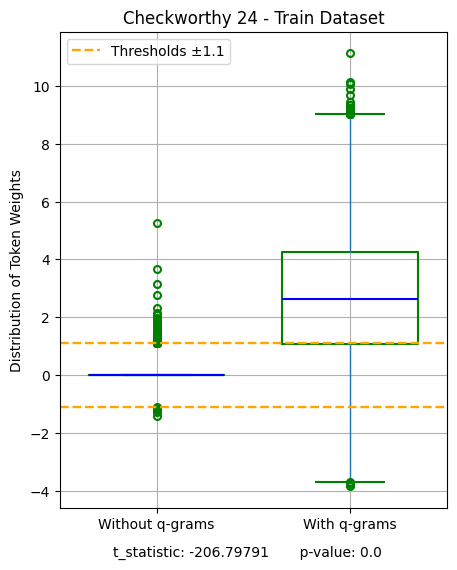
\includegraphics[width=\linewidth]{fig_checkworthy_24_train.png}
            \label{fig:image1}
        \end{subfigure} &
        \begin{subfigure}{0.32\textwidth}
            \centering
            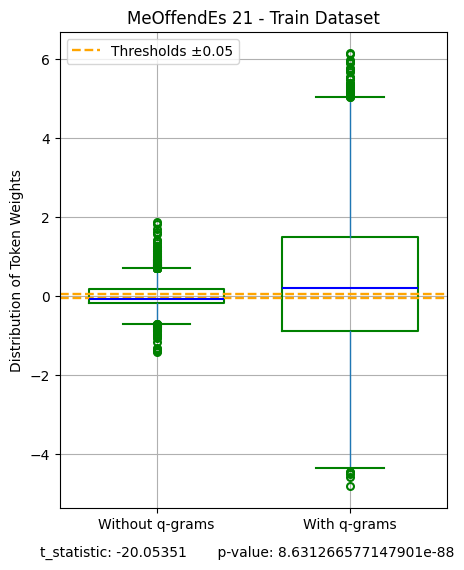
\includegraphics[width=\linewidth]{fig_meoffendes_21_train_0_05.png}
            \label{fig:image2}
        \end{subfigure} &
        \begin{subfigure}{0.32\textwidth}
            \centering
            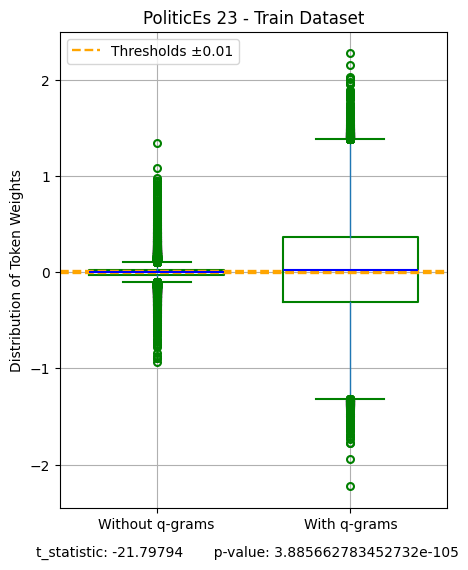
\includegraphics[width=\linewidth]{fig_politicses_23_train.png}
            \label{fig:image3}
        \end{subfigure}
    \end{tabular}

    % Espacio reducido entre filas
    \vspace{0.15cm}

    % Fila 2 - Test
    \begin{tabular}{c c c}
        \begin{subfigure}{0.32\textwidth}
            \centering
            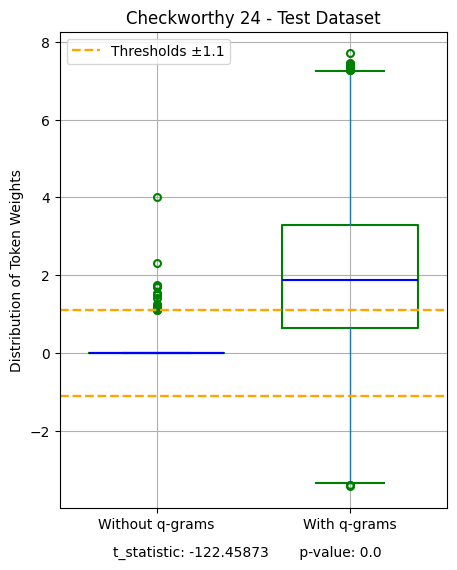
\includegraphics[width=\linewidth]{fig_checkworthy_24_test.png}
            \label{fig:image4}
        \end{subfigure} &
        \begin{subfigure}{0.32\textwidth}
            \centering
            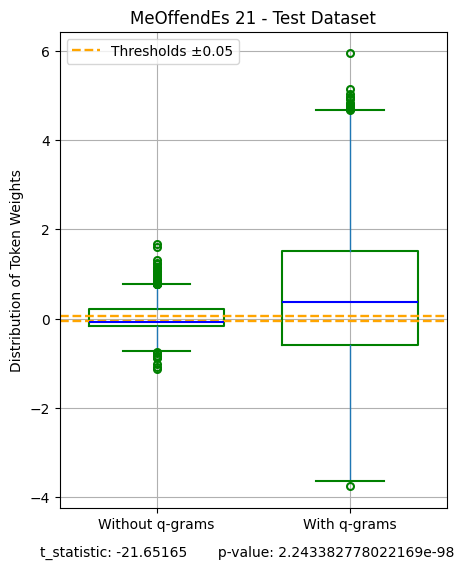
\includegraphics[width=\linewidth]{fig_meoffendes_21_test_0_05.png}
            \label{fig:image5}
        \end{subfigure} &
        \begin{subfigure}{0.32\textwidth}
            \centering
            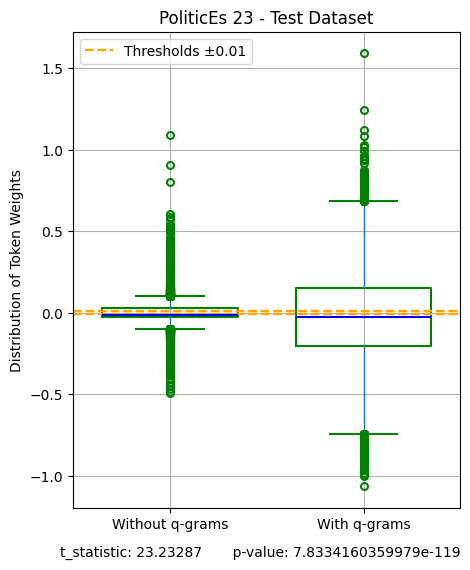
\includegraphics[width=\linewidth]{fig_politicses_23_test.png}
            \label{fig:image6}
        \end{subfigure}
    \end{tabular}

    \caption{Comparison of word importance distributions between Scenario~1 (word-level tokenization) and Scenario~2 (q-gram-based tokenization) across three datasets: \textit{CheckWorthiness}, \textit{MeOffendEs}, and \textit{PoliticEs}. The boxplots display the distribution of token weights for training and testing sets. A predefined threshold (dashed line) is used to identify tokens considered relevant for model interpretability. The results show that Scenario~2 consistently yields a greater number of tokens with weights outside the predefined threshold range, supporting the effectiveness of q-gram traceability.}

    \label{fig:fig_bloxplots}

\end{figure}


\subsection{Comparison with Post-Hoc Interpretability Methods}

Table~\ref{tab:comparison_methods} compares \ac{GWTI} with \ac{SHAP} and \ac{LIME}—tools within the broader domain of Explainable Artificial Intelligence (XAI)—. While \ac{SHAP} and \ac{LIME} are model-agnostic and work post-hoc, they suffer from high computational cost, limited scalability to thousands of tokens, and approximation noise in sparse settings. As discussed in subsection \ref{post-hoc-strengths} under \textit{Post-hoc Explainability: Strengths and Weaknesses}, these tools face significant challenges in high-dimensional, sparse textual spaces such as those produced by q-gram tokenization.

\begin{table}[ht]
    \centering
    \begin{tabular}{p{5cm}p{5cm}p{2cm}p{2cm}}
        \toprule
            \textbf{Criterion} & \textbf{GWTI (Proposed)} & \textbf{SHAP} & \textbf{LIME} \\
        \midrule
            \textbf{Interpretability Phase} & Pre-hoc (integrated into preprocessing) & Post-hoc & Post-hoc \\
            \textbf{Token-level Explanation} & Yes (via q-gram aggregation) & Approximate & Approximate \\
            \textbf{Linguistic Traceability} & Yes (q-gram $\rightarrow$ word mapping) & No & Limited \\
            \textbf{Computational Cost} & Low & High & Medium \\
            \textbf{Scalability to Many Instances} & High & Low & Low \\
            \textbf{Support for Sparse Data} & Native (TF-IDF + Linear Model) & Requires sampling & Requires sampling \\
            \textbf{Model Dependency} & Works best with linear models & Model-agnostic & Model-agnostic \\
        \bottomrule
    \end{tabular}
    \caption{Comparison Between the Proposed Approach (\ac{GWTI}) and Post-Hoc Methods. }
    \label{tab:comparison_methods}
\end{table}

% SHAP and LIME are well-known post-hoc interpretability methods. For a detailed discussion of their strengths and limitations, see~\cite{peeters2021exploring}

Specifically, \ac{SHAP} visualizations become cluttered or even unreadable when attempting to display the contribution of hundreds of q-grams per instance. This hinders their usefulness for tasks like tweet classification or user profiling, where short texts often yield extremely sparse feature sets.

\ac{GWTI}, by contrast, operates pre-hoc, is deterministic, and supports full-corpus visualizations with minimal overhead. It delivers fast, accurate token-level visualizations by leveraging the linear model's coefficients and \ac{mTc}’s traceable q-grams. This integrated approach enables better exploration, dataset refinement, and transparency before model deployment.

\section{Applications}
\ac{GWTI} extends beyond token-level interpretability, offering practical advantages in various stages of model development and data refinement. Its computational efficiency, visualization capabilities, and traceability mechanism support tasks commonly found in modern NLP workflows, particularly those involving short-text classification. Below, we summarize key application scenarios:

\subsubsection*{Active Learning and Uncertainty Sampling:} \ac{GWTI} highlights uncertain or borderline predictions via the decision function, enabling strategies like least-confidence and margin sampling. Its efficiency allows frequent model retraining, improving active learning cycles.

\subsubsection*{Error Analysis and Data Selection:} The interpretability maps help detect samples where the model overweighs irrelevant tokens or fails due to preprocessing issues. Analysts can identify misclassified or ambiguous examples, refine labels, and eliminate noisy instances.

\subsubsection*{Bias and Pattern Discovery:} By tracing q-gram influence, \ac{GWTI} reveals unexpected patterns or token-level biases, such as names or slurs disproportionately affecting outcomes. This supports model fairness evaluations and bias mitigation.

\subsubsection*{Domain Adaptation and Customization:} \ac{GWTI} helps compare interpretability across datasets. Analysts can adapt classifiers to new domains (e.g., medical, legal) by identifying shifts in key term relevance and adjusting feature weights.

\subsubsection*{Rapid Interpretability and Augmentation:} \ac{GWTI}'s lightweight tracing supports batch explanations, aiding quick dataset reviews and generation of synthetic instances. For example, analysts can produce counterfactuals by altering key tokens with high weights and observing predicted outcomes.

\subsubsection*{Conclusion:} \ac{GWTI} acts not only as a transparent interpretability tool but also as a strategic asset in active learning, dataset debugging, and adaptive modeling. Its pre-hoc structure, low computational overhead, and compatibility with sparse, short-text data make it particularly suitable for large-scale or resource-constrained NLP workflows.

\section{Discussion and Conclusion}
\label{sec/discussion}

The \ac{GWTI} framework was introduced to address the dual challenges of interpretability and computational efficiency in short-text NLP tasks. Through its integration of q-gram tokenization, a linear estimator, and a traceability mechanism, \ac{GWTI} generates clear, token-level visualizations that link subword features to human-readable words. This approach has demonstrated consistent advantages over post-hoc tools in sparse and high-dimensional contexts, such as tweet classification and user profiling.

Experimental evidence supports the hypothesis that q-gram traceability enhances model interpretability. \ac{GWTI} enables the identification of influential tokens that would otherwise remain hidden in traditional word-based schemes. In comparison to \ac{SHAP} and \ac{LIME}, \ac{GWTI} offers scalability, low computational cost, and corpus-level insight, positioning it as a practical solution for real-time inspection, error analysis, and active learning workflows.

The design of \ac{GWTI} remains intentionally lightweight. By relying on linear models and deterministic tokenization (\ac{mTc}), it ensures reproducible explanations and compatibility with resource-constrained environments. Moreover, its ability to trace feature contributions prior to model training enables a more efficient pipeline for dataset refinement and model debugging.

In summary, \ac{GWTI} provides a pre-hoc, interpretable, and computationally efficient framework tailored to short-text NLP. It supports scalable and reliable analysis, contributing not only to model transparency but also to improved robustness and data-centric model development.

\section{Future Work}

While \ac{GWTI} has shown promising results in enhancing interpretability for short-text NLP, several directions remain open for future research:

\begin{itemize}
    \item \textbf{Evaluate Impact on Target Models:} Future studies should measure how interpretability-driven data refinement using \ac{GWTI} influences the final performance of complex target models beyond linear baselines.
    
    \item \textbf{Extend Traceability Coverage:} Current tracing is limited to intra-word q-grams. Investigating strategies to incorporate q-grams that span across word boundaries or employ skip-grams could improve semantic coverage.
    
    \item \textbf{Adaptation to Non-Linear Models:} Although \ac{GWTI} is optimized for linear classifiers, its traceability and visualization pipeline may be adapted to deep learning architectures such as CNNs or Transformer-based models by integrating surrogate linear interpreters.
    
    \item \textbf{Enhance Visual and Structural Output:} Further improvements in the format, interactivity, or semantic structure of the interpretability output (e.g., nested views or semantic clustering of tokens) may increase usability for downstream research or industry pipelines.
    
    \item \textbf{Enable Real-Time Feedback for Annotation:} Integrating \ac{GWTI} into human-in-the-loop workflows for data labeling or active annotation may support real-time explainability feedback to guide annotators or accelerate training set improvements.
\end{itemize}

These directions aim to further expand the utility and generalizability of \ac{GWTI}, strengthening its role in interpretable, scalable, and human-centered machine learning.

\section*{Availability of Resources}

The source codes for the Interpretability by Gram-Weighted Tracing (\ac{GWTI}) framework, along with reproducible experiments, are publicly available in the GitHub repository at:

Not yet...

\section{Acknowledgements}
\paragraph{The first author thanks to MSc Rodrigo Dominguez and Professor Jacques Savoy for their invaluable comments and suggestions.} 

%\bibliographystyle{splncs04}
\bibliographystyle{elsarticle-num}
\bibliography{biblio.bib}

\newpage

\appendix

\section{Appendix: Example of JSON Structure Generated by the \ac{GWTI}}
\label{ap:example_structure}

Basic and trimmed example of an instance from a German tweet dataset.

\small
\begin{verbatim} 
{
    "101": {
        "prediction_klass": "1",
        "decision_value": "0.6579841325",
        "true_klass": "1",
        "data": {
            "restaurants": {
                "weight": 0.7325947434,
                "grams": {
                    "q:rest": 0.0358046721,
                    "q:taur": 0.0487939050
                },
                "color": "#FF0000"
            },
            "groningen": {
                "weight": 0.0179637958,
                "grams": {
                    "q:inge": 0.0212614873,
                    "q:gro": 0.0107364526
                },
                "color": "#FFC6C6"
            }
        }
    }
}
\end{verbatim}

\textbf{Explanation of the Example:} \\
The instance \texttt{"101"} represents a classification prediction with:

\begin{itemize}
    \item \textbf{Instance "101":}
    \begin{itemize}
        \item \textbf{prediction klass:} The predicted class by the model is "1".
        \item \textbf{decision value:} The decision value calculated for this instance is "0.6579841325", indicating the confidence level in the prediction.
        \item \textbf{true klass:} The actual class of the tweet is "1", useful for comparative evaluation.
    \end{itemize}
    \item \textbf{data (Details at the word and q-gram level):}
    \begin{itemize}
        \item \textbf{Word "restaurants":}
        \begin{itemize}
            \item \textbf{weight:} Total weight of the word is 0.7325947434, representing its contribution to the decision function.
            \item \textbf{grams:}
            \begin{itemize}
                \item \textbf{q:rest:} Contributes a weight of 0.0358046721.
                \item \textbf{q:taur:} Contributes a weight of 0.0487939050.
            \end{itemize}
            \item \textbf{color:} Assigned color is \#FF0000, which reflects the predicted class, with the intensity indicating the magnitude of the contribution to the prediction, facilitating interpretive visualization on the web interface.
        \end{itemize}
        \item \textbf{Word "\#groningen":}
        \begin{itemize}
            \item \textbf{weight:} Total weight of the word is 0.0179637958, representing its contribution to the decision function.
            \item \textbf{grams:}
            \begin{itemize}
                \item \textbf{q:inge:} Contributes a weight of 0.0212614873.
                \item \textbf{q:gro:} Contributes a weight of 0.0107364526.
            \end{itemize}
            \item \textbf{color:} Assigned color is \#FFC6C6, used to facilitate interpretive visualization on the web interface.           
        \end{itemize}
    \end{itemize}
\end{itemize}

\newpage

\section{Appendix: User Interface}
\label{ap:user_interface}

User Interface of the \ac{GWTI} Web Tool for Tweet Interpretability

\begin{figure}[htbp]
  %\centering
  \hspace*{-1.7cm}
  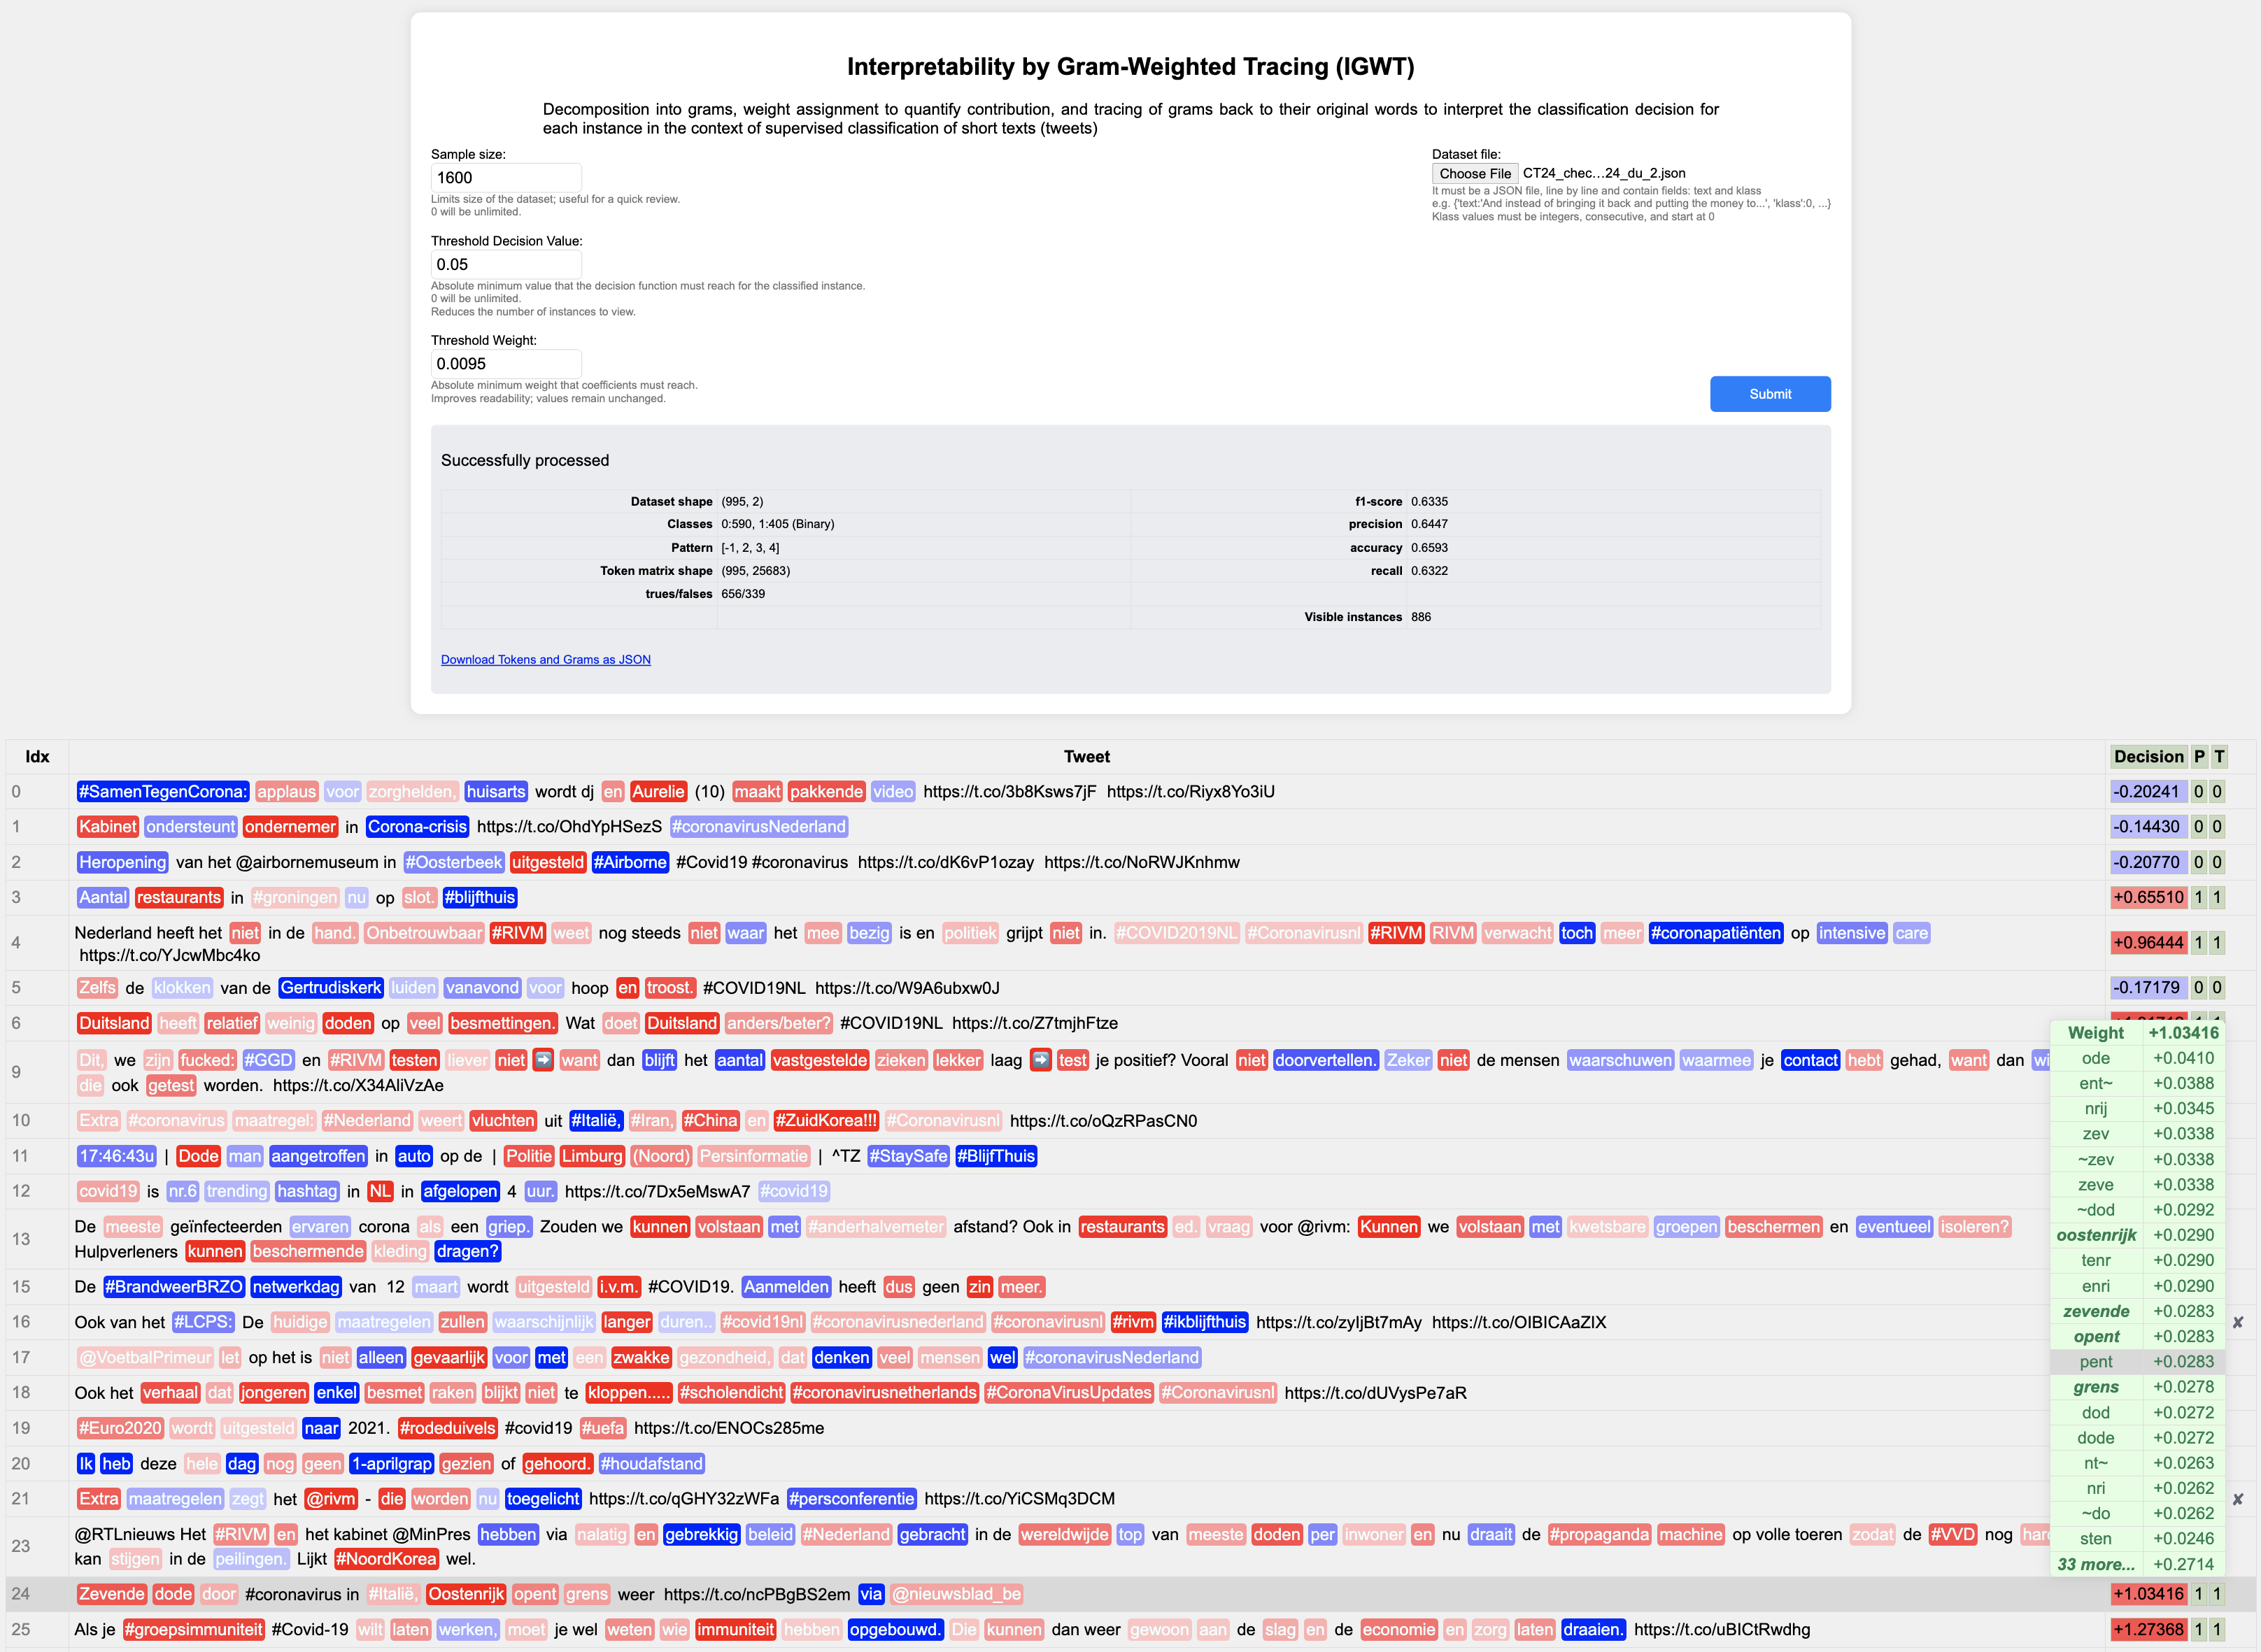
\includegraphics[width=1.2\textwidth]{big_screen.png}
  \label{fig:user_interface}
\end{figure}
  
\vspace*{-0.7cm}

Screenshot of the \ac{GWTI} web-based platform User Interface. It displays the input data: a dataset of tweets in German, the sample size, and the established thresholds. The metrics obtained with the LinearSVC surrogate model and the link to download the complete structure are clearly visible. In the instance space, 25 tweets out of the 886 filtered from a total of 995 are showcased. On the left, the breakdown of tokens and q-grams for instance number 24 is highlighted in green. Each instance features a color code varying according to the class and the intensity defined by the corresponding coefficient.

\end{document}
